\documentclass[11pt]{article}

% Increase main memory size
\usepackage{etex}
\usepackage{morewrites}
\usepackage{multicol}
\usepackage{pgfplots}
\usepackage{tikz}
\usetikzlibrary{external}
\tikzexternalize[prefix=cached_models/]

\usepackage{etex}
\usepackage{morewrites}
\usepackage{enumitem}
\usepackage{float}

\listfiles

\usepackage{amsmath, amssymb, amsthm}
\usepackage{graphicx}
\usepackage{geometry}
\usepackage{array}
\usepackage{booktabs}
\usepackage{float}
\usepackage{verbatim}
\usetikzlibrary{3d}

% Page Layout
\geometry{a4paper, margin=1in}
\setlength\parindent{0pt}
\pgfplotsset{compat=1.18}

% Custom commands
\newcommand{\card}[1]{\lvert #1 \rvert}
\newcommand{\inner}[2]{\left\langle #1, #2 \right\rangle}

\title{\textbf{Numerical Linear Algebra}}
\author{}
\date{}

\begin{document}

\maketitle

\section{Matrices, Vectors, and Norms}
\subsection{Matrix-Vector Multiplication}
Given a matrix \( A \in \mathbb{C}^{m \times n} \) and a vector \( x \in \mathbb{C}^n \), the matrix-vector product \( Ax = b \in \mathbb{C}^m \) is defined as:

\[
b_i = \sum_{j=1}^{n} a_{ij} x_j, \quad \text{for } i = 1, \ldots, m
\]

where \( a_{ij} \) are the entries of the matrix \( A \).

\subsubsection*{Observation}
The transformation \( x \mapsto Ax \) is a linear transformation from \( \mathbb{C}^n \) to \( \mathbb{C}^m \), i.e., it satisfies:
\[
A(x + y) = Ax + Ay, \quad A(\alpha x) = \alpha Ax, \quad \text{for all } x, y \in \mathbb{C}^n, \alpha \in \mathbb{C}
\]

\subsubsection{A Matrix times a Vector}
\[b = Ax = \sum_{j=1}^{n} x_j a_j\]
where \( a_j \) is the \( j \)-th column of \( A \).

\[\begin{bmatrix}
b_1 \\
b_2 \\
\vdots \\
b_m
\end{bmatrix} =
\begin{bmatrix}
a_{11} & a_{12} & \cdots & a_{1n} \\
a_{21} & a_{22} & \cdots & a_{2n} \\
\vdots & \vdots & \ddots & \vdots \\
a_{m1} & a_{m2} & \cdots & a_{mn}
\end{bmatrix}
\begin{bmatrix}
x_1 \\
x_2 \\
\vdots \\
x_n
\end{bmatrix} =
x_1
\begin{bmatrix}
a_{11} \\
a_{21} \\
\vdots \\
a_{m1}
\end{bmatrix} +
x_2
\begin{bmatrix}
a_{12} \\
a_{22} \\
\vdots \\
a_{m2}
\end{bmatrix} + \cdots +
x_n
\begin{bmatrix}
a_{1n} \\
a_{2n} \\
\vdots \\
a_{mn}
\end{bmatrix}\]

\subsubsection*{Example: Vandermonde Matrix}
A Vandermonde matrix is defined as:
\[
A = \begin{bmatrix}
1 & x_1 & x_1^2 & \cdots & x_1^{n-1} \\
1 & x_2 & x_2^2 & \cdots & x_2^{n-1} \\
\vdots & \vdots & \vdots & \ddots & \vdots \\
1 & x_m & x_m^2 & \cdots & x_m^{n-1}
\end{bmatrix} \in \mathbb{C}^{m \times n}
\]

\subsubsection*{Observation}
Let fix the sequence \( \{x_1, x_2, \ldots, x_m \} \). If $p$ and $q$ are polynomials of degree at most $n-1$ and $\alpha$ is a scalar, then:
\begin{enumerate}
    \item $(p + q)$ is a polynomial of degree at most $n-1$, and so are $\alpha p, \alpha q$.
    \item $(p + q)(x_i) = p(x_i) + q(x_i)$ for $i = 1, \ldots, m$.
    \item $(\alpha p)(x_i) = \alpha p(x_i)$ for $i = 1, \ldots, m$.
\end{enumerate}

\subsubsection*{Observation}
Suppose we have a vector \( c \in \mathbb{C}^n \) representing the coefficients of a polynomial \( p(x) = c_0 + c_1 x + c_2 x^2 + \cdots + c_{n-1} x^{n-1} \). Then 
\[p(x_i) = (Ac)_i = c_0 + c_1 x_i + c_2 x_i^2 + \cdots + c_{n-1} x_i^{n-1}\]

Any polynomial of degree at most \( n-1 \) can be represented as
\[p(x) = \begin{bmatrix}
1 & x & x^2 & \cdots & x^{n-1}
\end{bmatrix}
\begin{bmatrix}
c_0 \\
c_1 \\
c_2 \\
\vdots \\
c_{n-1}
\end{bmatrix}
\]

\subsection{Matrix-Matrix Multiplication}
Given matrices \( A \in \mathbb{C}^{l \times m} \) and \( C \in \mathbb{C}^{m \times n} \), the matrix-matrix product \( B = AC \in \mathbb{C}^{l \times n} \) is defined as:

\[
b_{ij} = \sum_{k=1}^{m} a_{ik} c_{kj}, \quad \text{for } i = 1, \ldots, l, j = 1, \ldots, n
\]

So,
\[B = \begin{bmatrix}
b_1 & b_2 & \cdots & b_n
\end{bmatrix} = \begin{bmatrix}
a_1 & a_2 & \cdots & a_m
\end{bmatrix} \begin{bmatrix}
c_1 & c_2 & \cdots & c_n
\end{bmatrix}\]
\[b_j = Ac_j = \sum_{k=1}^{m} c_{kj} a_k, \quad j = 1, \ldots, n\]

\subsubsection*{Example: Outer Product}
Given two vectors \( u \in \mathbb{C}^{m\times 1} \) and \( v \in \mathbb{C}^{1\times n} \), the outer product \( uv^T \in \mathbb{C}^{m \times n} \) is defined as:
\[\begin{bmatrix}
    u_1 \\
    u_2 \\
    \vdots \\
    u_m
\end{bmatrix}
\begin{bmatrix}
    v_1 & v_2 & \cdots & v_n
\end{bmatrix} = \begin{bmatrix}
    u_1 v_1 & u_1 v_2 & \cdots & u_1 v_n \\
    u_2 v_1 & u_2 v_2 & \cdots & u_2 v_n \\
    \vdots & \vdots & \ddots & \vdots \\
    u_m v_1 & u_m v_2 & \cdots & u_m v_n
\end{bmatrix}
\]

\subsubsection*{Example}
Let \( B \in \mathbb{C}^{m \times n} \), let \( a_1, a_2, \ldots, a_n \) be the columns of \( A \in \mathbb{C}^{m \times n} \) and let \( R \in \mathbb{C}^{n \times n} \) be an upper triangular matrix with all its superdiagonal entries equal to 1 such that
\[B = \begin{bmatrix}
    b_1 & b_2 & \dots & b_n
\end{bmatrix} = \begin{bmatrix}
    a_1 & a_2 & \dots & a_n
\end{bmatrix} \begin{bmatrix}
    1 & 1 & \dots & 1 \\
    0 & 1 & \dots & 1 \\
    \vdots & \vdots & \ddots & \vdots \\
    0 & 0 & \dots & 1
\end{bmatrix}\]
Then,
\[b_j = A r_j = \sum_{k=1}^{j} a_k, \quad j = 1, \ldots, n\] 
which is known as the indefinite integral operation.

\subsection{Range and Null Space}
\subsubsection*{Theorem}
The range of a matrix \( A \in \mathbb{C}^{m \times n} \) is the space spanned by its columns, i.e. it's column space.
\begin{quotation}
    \textit{"The set of vectors that can be written as \( Ax \) for some \( x \in \mathbb{C}^n \)."}
\end{quotation}

\subsubsection{Null Space and Rank}
The null space of a matrix \( A \in \mathbb{C}^{m \times n} \) is defined as:
\[\text{span} \{x \in \mathbb{C}^n : Ax = 0\}\]

The rank of a matrix \( A \in \mathbb{C}^{m \times n} \) is defined as the dimension of its range:
\[\text{rank}(A) = \dim(\text{range}(A))\]

\subsubsection*{Theorem}
For any matrix \( A \in \mathbb{C}^{m \times n}, m \geq n \), \( A \) has full rank if and only if it maps no two distinct vectors to the same vector:
\[Ax = Ay \implies x = y, \forall x, y \in \mathbb{C}^n \quad \text{and} \quad Ax \neq Ay \implies x \neq y, \forall x, y \in \mathbb{C}^n\]

\subsubsection{Non-singular Matrices}
A non-singular matrix, or invertible matrix is a square matrix \( A \in \mathbb{C}^{n \times n} \) that has full rank.

\subsubsection{Inverse of a Matrix}
The matrix \( A \in \mathbb{C}^{n \times n} \) is the inverse of \( Z \) if and only if:
\[AZ = ZA = I = \begin{bmatrix}
    e_1 & e_2 & \cdots & e_n
\end{bmatrix}\]
where \( e_i \) is the \( i \)-th standard basis vector. Furthermore, the inverse of a matrix is unique and
\[\text{rank}(A) = n = \text{rank}(Z)\]

\subsubsection*{Theorem}
For $A \in \mathbb{C}^{n \times n}$, the following statements are equivalent:
\begin{enumerate}
    \item $A$ has an inverse $A^{-1}$.
    \item $A$ has full rank, i.e. $\text{rank}(A) = n$.
    \item The columns of $A$ span $\mathbb{C}^n$, i.e. $\text{range}(A) = \mathbb{C}^n$.
    \item The columns of $A$ are linearly independent, i.e. $\text{null}(A) = \{0\}$.
    \item $0$ is not an eigenvalue of $A$.
    \item $0$ is not a singular value of $A$.
    \item $\card{A} \neq 0$.
\end{enumerate}

\subsection{Orthogonal Vectors and Matrices}
\subsubsection{Complex Conjugate and Conjugate Transpose}
Given $z \in \mathbb{C}$, the complex conjugate of $z$ is denoted by $\bar{z}$ or $z^*$, where if $z = x + iy$, then $\bar{z} = x - iy$.

The conjugate transpose of a matrix $A \in \mathbb{C}^{m \times n}$ is denoted by $A^*$, where $A^* = \bar{A}^T$.
\[A = \begin{bmatrix}
    a_{11} & a_{12} \\
    a_{21} & a_{22} \\
    a_{31} & a_{32} \\
\end{bmatrix} \implies A^* = \begin{bmatrix}
    \bar{a}_{11} & \bar{a}_{21} & \bar{a}_{31} \\
    \bar{a}_{12} & \bar{a}_{22} & \bar{a}_{32} \\
\end{bmatrix}\]

\subsubsection{Hermitian Matrices and Skew-Hermitian Matrices}
A matrix $A \in \mathbb{C}^{n \times n}$ is called Hermitian if $A^* = A$. (Or $A = A^T$ if $A \in \mathbb{R}^{n \times n}$.)

A matrix $A \in \mathbb{C}^{n \times n}$ is called Skew-Hermitian if $A^* = -A$. (Or $A = -A^T$ if $A \in \mathbb{R}^{n \times n}$.)

\subsubsection{Inner Product and Norm}
Given two vectors $x, y \in \mathbb{C}^n$, the inner product is defined as:
\[\inner{x}{y} = y^* x = \sum_{i=1}^{n} \bar{y}_i x_i\]

The norm of a vector $x \in \mathbb{C}^n$ is defined as:
\[\|x\| = \sqrt{\inner{x}{x}} = \sqrt{\sum_{i=1}^{n} |x_i|^2}\]

The modulus of a complex number $z \in \mathbb{C}$ is defined as:
\[|z| = \sqrt{z \bar{z}} = \sqrt{x^2 + y^2} \quad \text{where } z = x + iy\]

The angle $\theta$ between two vectors $x, y \in \mathbb{C}^n$ is defined as:
\[\cos(\theta) = \frac{\inner{x}{y}}{\|x\| \|y\|}\]

\subsubsection*{Observation}
The inner product is bilinear, which means:
\begin{enumerate}
    \item $\inner{x_1 + x_2}{y} = \inner{x_1}{y} + \inner{x_2}{y}$
    \item $\inner{x}{y_1 + y_2} = \inner{x}{y_1} + \inner{x}{y_2}$
    \item $\inner{\alpha x}{\beta y} = \alpha \bar{\beta} \inner{x}{y}$ for all $\alpha, \beta \in \mathbb{C}$
\end{enumerate}

For all vectors or matrices $A, B$ of compatible dimensions, we have:
\[(A B)^* = B^* A^*\]

\subsubsection{Orthogonal Vectors}
Two vectors $x, y \in \mathbb{C}^n$ are orthogonal if $\inner{x}{y} = 0$.

\subsubsection*{Observation}
If $x$ and $y$ are orthogonal, then they are perpendicular.

With $x = \{x_1, x_2, \ldots, x_n\}$ and $y = \{y_1, y_2, \ldots, y_n\}$, $x$ and $y$ are orthogonal if and only if:
\[\inner{x_i}{y_j} = 0, \quad \forall i, j = 1, 2, \ldots, n\]

\subsubsection{Orthonormal Vectors}
A set of vectors $\{x_1, x_2, \ldots, x_n\} \subset \mathbb{C}^n$ is orthonormal if:
\[\inner{x_i}{x_j} = 0 \text{ for } i \neq j \quad \text{and} \quad \inner{x_i}{x_i} = \|x_i\|^2 = 1\]

\subsubsection*{Observation}
The vectors in an orthogonal set are linearly independent.

\subsubsection{Orthogonal and Unitary Matrices}
A matrix $Q \in \mathbb{R}^{n \times n}$ is orthogonal if its columns form an orthonormal set, i.e. $Q^T Q = QQ^T = I$.

A matrix $U \in \mathbb{C}^{n \times n}$ is unitary if its columns form an orthonormal set, i.e. $U^* U = UU^* = I$.

\subsubsection*{Observation}
If $U \in \mathbb{C}^{n \times n}$ is unitary, then $U^{-1} = U^*$ and 
\[\begin{bmatrix}
    u_1^* \\
    u_2^* \\
    \vdots \\
    u_n^*
\end{bmatrix} \begin{bmatrix}
    u_1 & u_2 & \cdots & u_n
\end{bmatrix} = \begin{bmatrix}
    1 & 0 & \cdots & 0 \\
    0 & 1 & \cdots & 0 \\
    \vdots & \vdots & \ddots & \vdots \\
    0 & 0 & \cdots & 1
\end{bmatrix}
\] 
which implies that $\inner{u_i}{u_j} = \delta_{ij}$ where $\delta_{ij}$ is the Kronecker delta, i.e. $\delta_{ij} = \begin{cases}
1 & \text{if } i = j \\
0 & \text{if } i \neq j
\end{cases}$.

\section{Vector Spaces}
A vector space $\mathcal{V}$ over a field $\mathbb{F}$ (usually $\mathbb{R}$ or $\mathbb{C}$) is a set of objects called vectors, along with two operations: vector addition and scalar multiplication, satisfying the following axioms for all $u, v, w \in \mathcal{V}$ and $\alpha, \beta \in \mathbb{F}$:
\begin{enumerate}
    \item (Closure under addition) $u + v \in \mathcal{V}$
    \item (Commutativity) $u + v = v + u$
    \item (Associativity) $(u + v) + w = u + (v + w)$
    \item (Existence of additive identity) There exists an element $0 \in \mathcal{V}$ such that $u + 0 = u$
    \item (Existence of additive inverses) For each $u \in \mathcal{V}$, there exists an element $-u \in \mathcal{V}$ such that $u + (-u) = 0$
    \item (Closure under scalar multiplication) $\alpha u \in \mathcal{V}$
    \item (Distributivity of scalar multiplication with respect to vector addition) $\alpha (u + v) = \alpha u + \alpha v$
    \item (Distributivity of scalar multiplication with respect to field addition) $(\alpha + \beta) u = \alpha u + \beta u$
    \item (Associativity of scalar multiplication) $\alpha (\beta u) = (\alpha \beta) u$
    \item (Existence of multiplicative identity) $1 u = u$ where $1$ is the multiplicative identity in $\mathbb{F}$
\end{enumerate}

\subsection{Linear Subspaces}
A subset $\mathcal{W}$ of a vector space $\mathcal{V}$ is a subspace if $\mathcal{W}$ is itself a vector space under the operations of addition and scalar multiplication defined on $\mathcal{V}$:
\begin{enumerate}
    \item (Closure under addition) $u + v \in \mathcal{W}$
    \item (Closure under scalar multiplication) $\alpha u \in \mathcal{W}$
\end{enumerate}

\subsection{Linear Independence}
A set of vectors $\{v_1, v_2, \ldots, v_k\} \subset \mathcal{V}$ is linearly independent if the only solution to
\[\alpha_1 v_1 + \alpha_2 v_2 + \cdots + \alpha_k v_k = 0\]
is $\alpha_1 = \alpha_2 = \cdots = \alpha_k = 0$. If there exists a non-trivial solution, the set is linearly dependent.

\subsection{Basis and Dimension}
A basis of a vector space $\mathcal{V}$ is a set of linearly independent vectors that spans $\mathcal{V}$. The dimension of $\mathcal{V}$, denoted $\dim(\mathcal{V})$, is the number of vectors in any basis of $\mathcal{V}$. 

\subsection{Inner Product and Norms}
An inner product on a vector space $\mathcal{V}$ over $\mathbb{F}$ is a function $\inner{\cdot}{\cdot} : \mathcal{V} \times \mathcal{V} \to \mathbb{F}$. The standard inner product on $\mathbb{C}^n$ is defined as:
\[\inner{x}{y} = y^* x = \sum_{i=1}^{n} \bar{y}_i x_i\]

A norm on a vector space $\mathcal{V}$ is a function $\|\cdot\| : \mathcal{V} \to \mathbb{R}$ satisfying:
\begin{enumerate}
    \item (Non-negativity) $\|v\| \geq 0$
    \item (Definiteness) $\|v\| = 0$ if and only if $v = 0$
    \item (Homogeneity) $\|\alpha v\| = |\alpha| \|v\|$ for all $\alpha \in \mathbb{F}$ and $v \in \mathcal{V}$
    \item (Triangle inequality) $\|u + v\| \leq \|u\| + \|v\|$ for all $u, v \in \mathcal{V}$
\end{enumerate}
The $p$-norm on $\mathbb{C}^n$ is defined as:
\[\|x\|_p = \left( \sum_{i=1}^{n} |x_i|^p \right)^{1/p}\]
for $1 \leq p < \infty$, and the $\infty$-norm is defined as:
\[\|x\|_\infty = \max_{1 \leq i \leq n} |x_i|\]

\begin{center}
    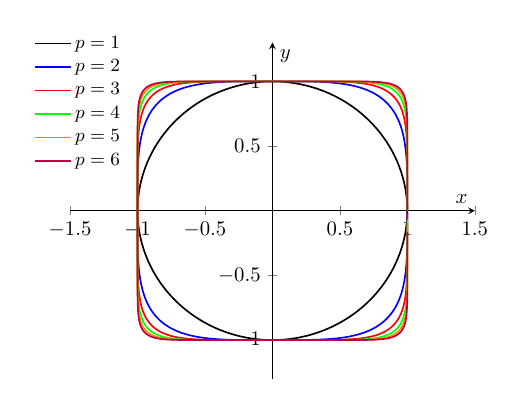
\begin{tikzpicture}[scale=0.75]
        \begin{axis}[
            axis lines = middle,
            xlabel = $x$,
            ylabel = {$y$},
            xmin=-1.5, xmax=1.5,
            ymin=-1.3, ymax=1.3,
            legend style={at={(0.15,0.6)}, anchor=south east, font=\small, draw=none, }
                ]       \addplot [
            domain=0:360, 
            samples=200, 
            smooth, 
            variable=\t, 
            thick,
            black
        ] 
        plot ({cos(\t)}, {sin(\t)});
        \addlegendentry{$p=1$}    
        \addplot [
            domain=0:360, 
            samples=200, 
            smooth, 
            variable=\t, 
            thick,
            blue
        ] 
        plot ({sign(cos(\t))*abs(cos(\t))^(1/2)}, {sign(sin(\t))*abs(sin(\t))^(1/2)});
        \addlegendentry{$p=2$}
        \addplot [
            domain=0:360, 
            samples=200, 
            smooth, 
            variable=\t, 
            thick,
            red
        ] 
        plot ({sign(cos(\t))*abs(cos(\t))^(1/3)}, {sign(sin(\t))*abs(sin(\t))^(1/3)});
        \addlegendentry{$p=3$}
        \addplot [
            domain=0:360, 
            samples=200, 
            smooth, 
            variable=\t, 
            thick,
            green
        ] 
        plot ({sign(cos(\t))*abs(cos(\t))^(1/4)}, {sign(sin(\t))*abs(sin(\t))^(1/4)});
        \addlegendentry{$p=4$}
        \addplot [
            domain=0:360, 
            samples=200, 
            smooth, 
            variable=\t, 
            thick,
            orange
        ] 
        plot ({sign(cos(\t))*abs(cos(\t))^(1/5)}, {sign(sin(\t))*abs(sin(\t))^(1/5)});
        \addlegendentry{$p=5$}
        \addplot [
            domain=0:360, 
            samples=200, 
            smooth, 
            variable=\t, 
            thick,
            purple
        ] 
        plot ({sign(cos(\t))*abs(cos(\t))^(1/6)}, {sign(sin(\t))*abs(sin(\t))^(1/6)});
        \addlegendentry{$p=6$}
        \end{axis}
    \end{tikzpicture}
    \hspace{1cm}
    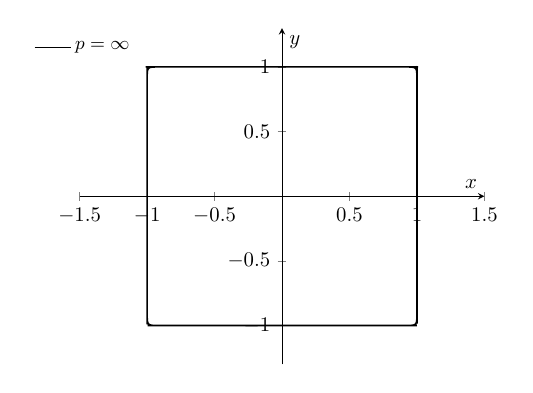
\begin{tikzpicture}[scale=0.75]
        \begin{axis}[
            axis lines = middle,
            xlabel = $x$,
            ylabel = {$y$},
            xmin=-1.5, xmax=1.5,
            ymin=-1.3, ymax=1.3,
            legend pos=north west,
            legend style={font=\small, draw=none, at={(0.15,0.9)}, anchor=south east}
        ]
        \addplot [
            domain=0:500, 
            samples=200, 
            smooth, 
            variable=\t, 
            thick,
            black
        ] 
        ({sign(cos(\t))*abs(cos(\t))^(1/30)}, {sign(sin(\t))*abs(sin(\t))^(1/30)});
        \addlegendentry{$p=\infty$}
        \end{axis} 
    \end{tikzpicture}
\end{center}

\subsubsection{Lemma}
Let $\|\cdot\|_\alpha$ and $\|\cdot\|_\beta$ be two norms on a finite-dimensional vector space $\mathcal{V}$. Then there exist positive constants $c_1$ and $c_2$ such that for all $v \in \mathcal{V}$:
\[c_1 \|v\|_\alpha \leq \|v\|_\beta \leq c_2 \|v\|_\alpha\]

$\|\cdot\|_\alpha$ and $\|\cdot\|_\beta$ are said to be equivalent norms. In $\mathbb{R}^n$:
\[\|x\|_2 \leq \|x\|_1 \leq \sqrt{n} \|x\|_2\]
\[\|x\|_\infty \leq \|x\|_2 \leq \sqrt{n} \|x\|_\infty\]
\[\|x\|_\infty \leq \|x\|_1 \leq n \|x\|_\infty\]

\section{Matrix Norms}
A matrix norm is a function $\|\cdot\| : \mathbb{C}^{m \times n} \to \mathbb{R}$ satisfying:
\begin{enumerate}
    \item (Non-negativity) $\|A\| \geq 0$
    \item (Definiteness) $\|A\| = 0$ if and only if $A = 0$
    \item (Homogeneity) $\|\alpha A\| = |\alpha| \|A\|$ for all $\alpha \in \mathbb{C}$ and $A \in \mathbb{C}^{m \times n}$ 
    \item (Triangle inequality) $\|A + B\| \leq \|A\| + \|B\|$ for all $A, B \in \mathbb{C}^{m \times n}$
    \item (Sub-multiplicativity) $\|AB\| \leq \|A\| \|B\|$ for all $A \in \mathbb{C}^{m \times n}$ and $B \in \mathbb{C}^{n \times p}$
\end{enumerate}

\subsection{Frobenius Norm}
The Frobenius norm of a matrix $A \in \mathbb{C}^{m \times n}$ is defined as:
\[\|A\|_F = \sqrt{\sum_{i=1}^{m} \sum_{j=1}^{n} |a_{ij}|^2} = \sqrt{\text{trace}(A^* A)}\]

\subsection{Induced Norms}
The induced norm (or operator norm) of a matrix $A \in \mathbb{C}^{m \times n}$ is defined as:
\[\|A\| = \sup_{x \neq 0} \frac{\|Ax\|}{\|x\|} = \sup_{\|x\| = 1} \|Ax\|\]  

\subsection{Consistent Norms}
Let $\|\cdot\|_{m \times n}, \|\cdot\|_{n \times p}$ and $\|\cdot\|_{m \times p}$ be three matrix norms on $\mathbb{C}^{m \times n}, \mathbb{C}^{n \times p}$ and $\mathbb{C}^{m \times p}$ respectively. They are said to be consistent if:
\[\|AB\|_{m \times p} \leq \|A\|_{m \times n} \|B\|_{n \times p}, \quad \forall A \in \mathbb{C}^{m \times n}, B \in \mathbb{C}^{n \times p}\]

\subsection{Properties of Induced Norms}
\begin{enumerate}
    \item $\|Ax\| \leq \|A\| \|x\|$ for all $A \in \mathbb{C}^{m \times n}$ and $x \in \mathbb{C}^n$
    \item $\|AB\| \leq \|A\| \|B\|$ for all $A \in \mathbb{C}^{m \times n}$ and $B \in \mathbb{C}^{n \times p}$
    \item $\|A\|_\infty = \max_{1 \leq i \leq m} \sum_{j=1}^{n} |a_{ij}|$ (maximum absolute row sum)
    \item $\|A\|_1 = \max_{1 \leq j \leq n} \sum_{i=1}^{m} |a_{ij}|$ (maximum absolute column sum)
    \item $\|A\|_2 = \sqrt{\lambda_{\max}(A^* A)}$ (with $\lambda_{\max}$ the largest eigenvalue)
    \item $\|A\|_2 = \|A^T\|_2$
    \item $\|A\|_2 = \max |\lambda_i(A)|$ if $A$ is normal (i.e. $A^* A = A A^*$)
    \item $\|A\|_F = \sqrt{\text{trace}(A^* A)}$
\end{enumerate} 

So, in general,
\[\|A\|_\alpha = \max_{x \neq 0} \frac{\|Ax\|_\alpha}{\|x\|_\alpha} = \max_{\|x\|_\alpha = 1} \|Ax\|_\alpha\]

The Frobenius norm is consistent with the euclidean vector norm, but it is not an induced norm.


\end{document}